
% This LaTeX was auto-generated from an M-file by MATLAB.
% To make changes, update the M-file and republish this document.

\documentclass{article}
\usepackage{graphicx}
\usepackage{color}

\sloppy
\definecolor{lightgray}{gray}{0.5}
\setlength{\parindent}{10pt}
\usepackage[margin=1in]{geometry}

\begin{document}

\title{Dynamical Adaptation in ORNs}
\author{Srinivas Gorur-Shandilya}
\maketitle

    
    
\subsection*{Contents}

\begin{itemize}
\setlength{\itemsep}{-1ex}
   \item Do ORNs rapidly modulate gain?
   \item Can the DA Model account for fast adaptation?
\end{itemize}


\subsection*{Do ORNs rapidly modulate gain?}

\begin{par}
Pseudo-white-noise analysis of ORN responses involves presenting binary flickering pulses of odor to the ORN and recording their response. If ORNs rapidly modulate gain on the timescale of response, then responses to pulses of odor in the sequence where the stimulus is locally low will be different from responses to pulses of odor in the sequence where the stimulus is locally high.
\end{par} \vspace{1em}
\begin{par}
The data looks like this. The following figure shows the valve state, the odor concentration, and the neuron response. The neuron is ab3A, and the odor presented is 1-octen-3-ol diluted to 3x $10^{-3}$ in Paraffin Oil. The correlation time in the valve position is 30ms.
\end{par} \vspace{1em}
\begin{par}
This data file is used for the following analysis:
\end{par} \vspace{1em}

        \color{lightgray} \begin{verbatim}final_2011_06_14_ab3A_1o3ol3X-3_20ml_30sec_30ms_rand.mat
\end{verbatim} \color{black}
    
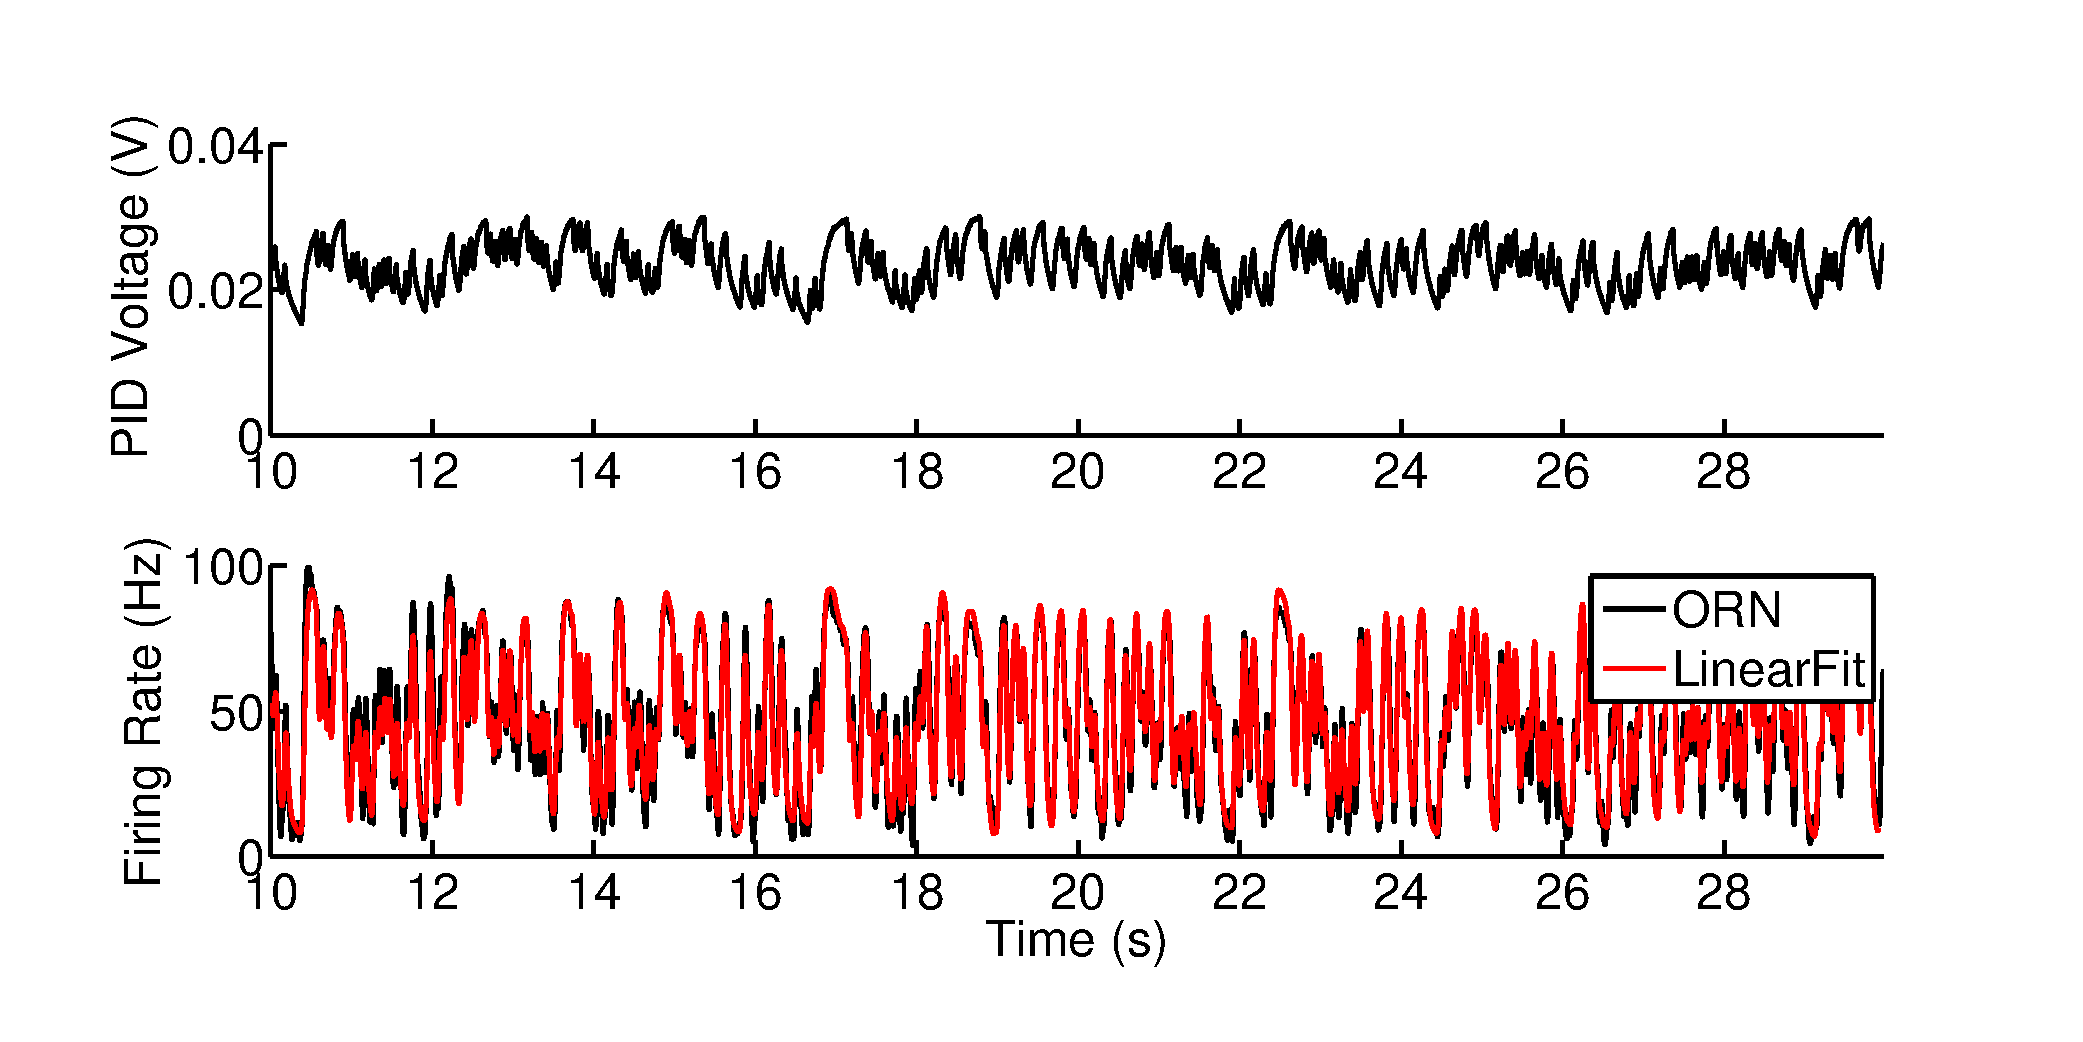
\includegraphics [width=\textwidth]{DA_Paper_01.pdf}

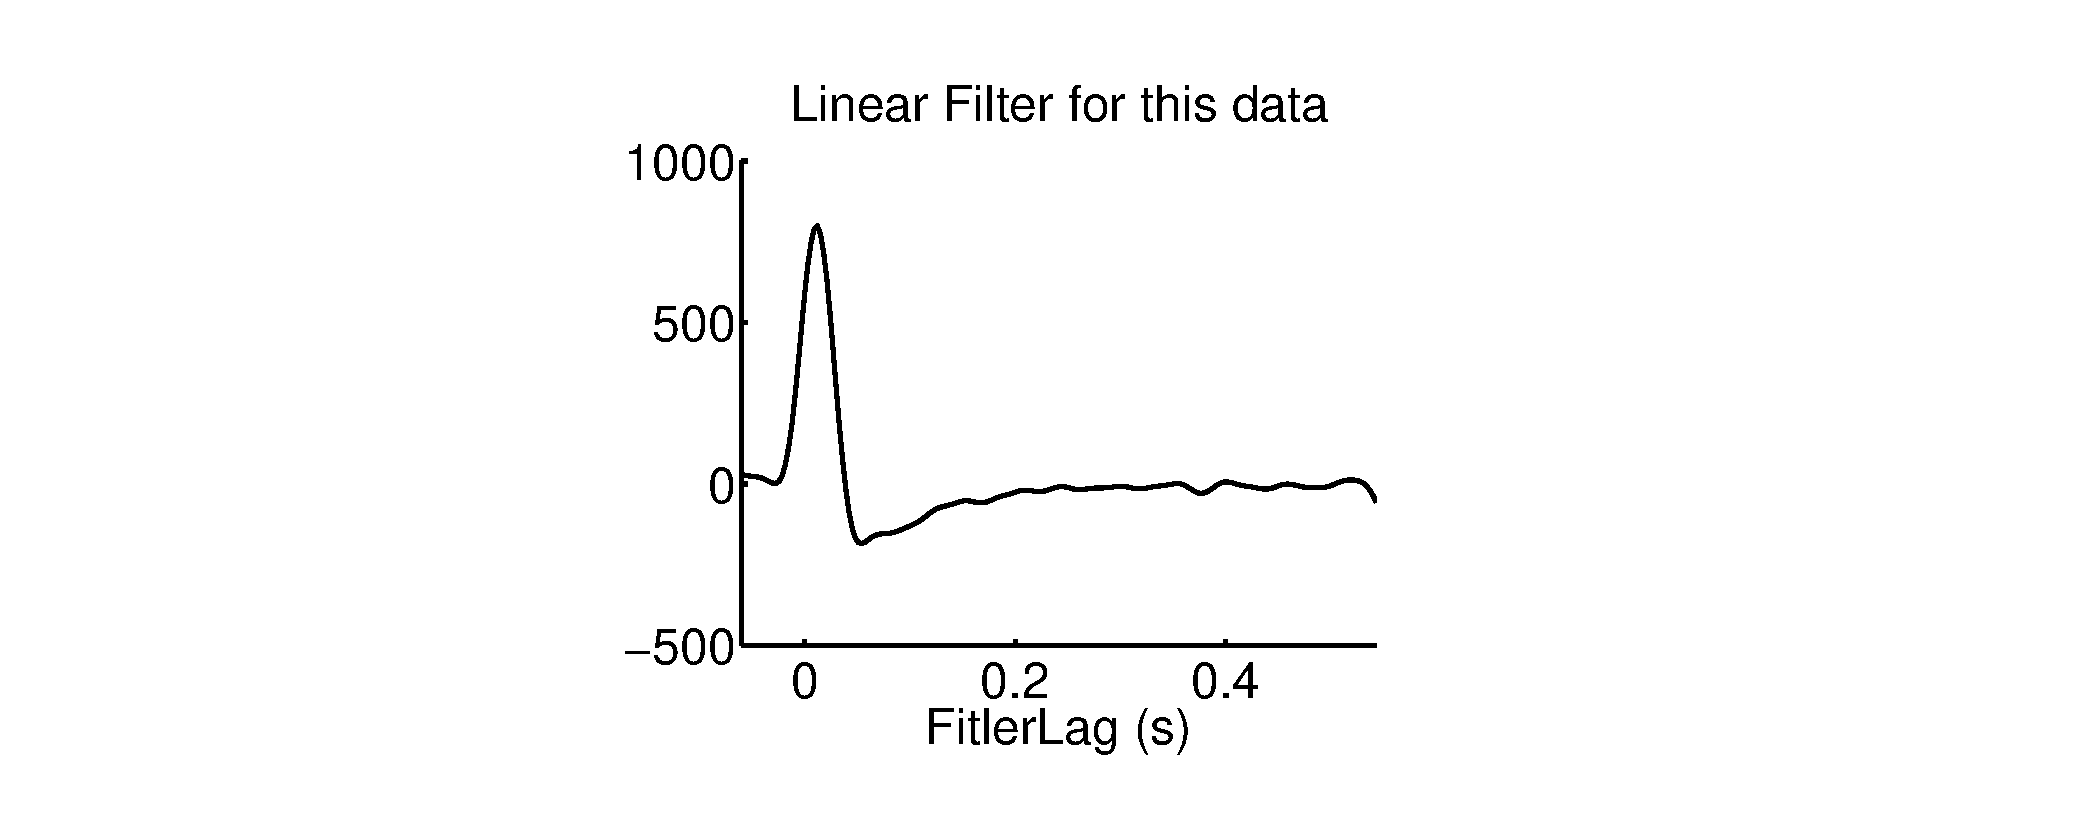
\includegraphics [width=\textwidth]{DA_Paper_02.pdf}
\begin{par}
The distributions of the input to neuron and the neuron responses are shown below on the left. The autocorrelaiton functions of the input and output are shown on the right. If the ORN modulates its gain on a rapid time-scale, it must do so in this case on a time-scale smaller than the autocorrelation time of the stimulus.
\end{par} \vspace{1em}

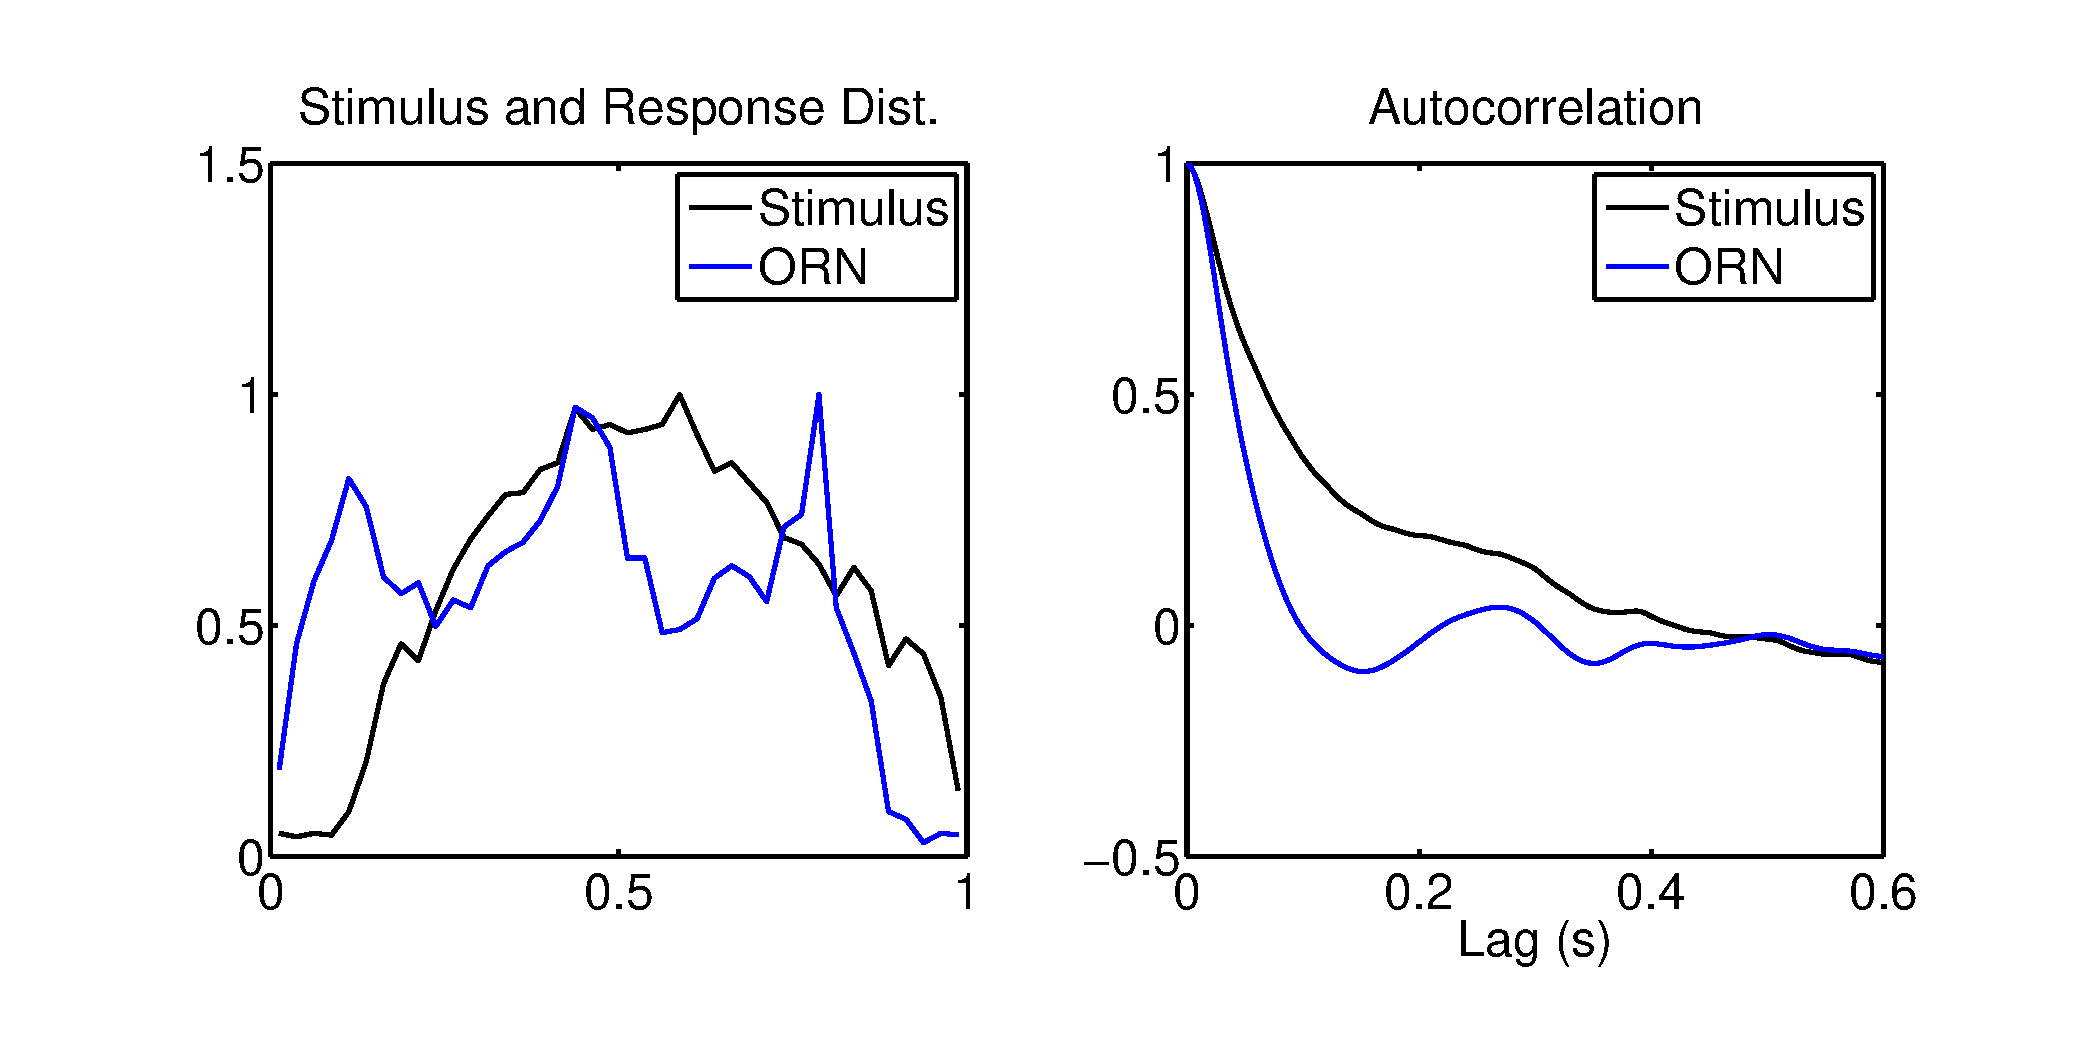
\includegraphics [width=\textwidth]{DA_Paper_03.pdf}
\begin{par}
Does the ORN selectively amplify responses to relatively small stimuli and suppress responses to relatively high stimuli?
\end{par} \vspace{1em}

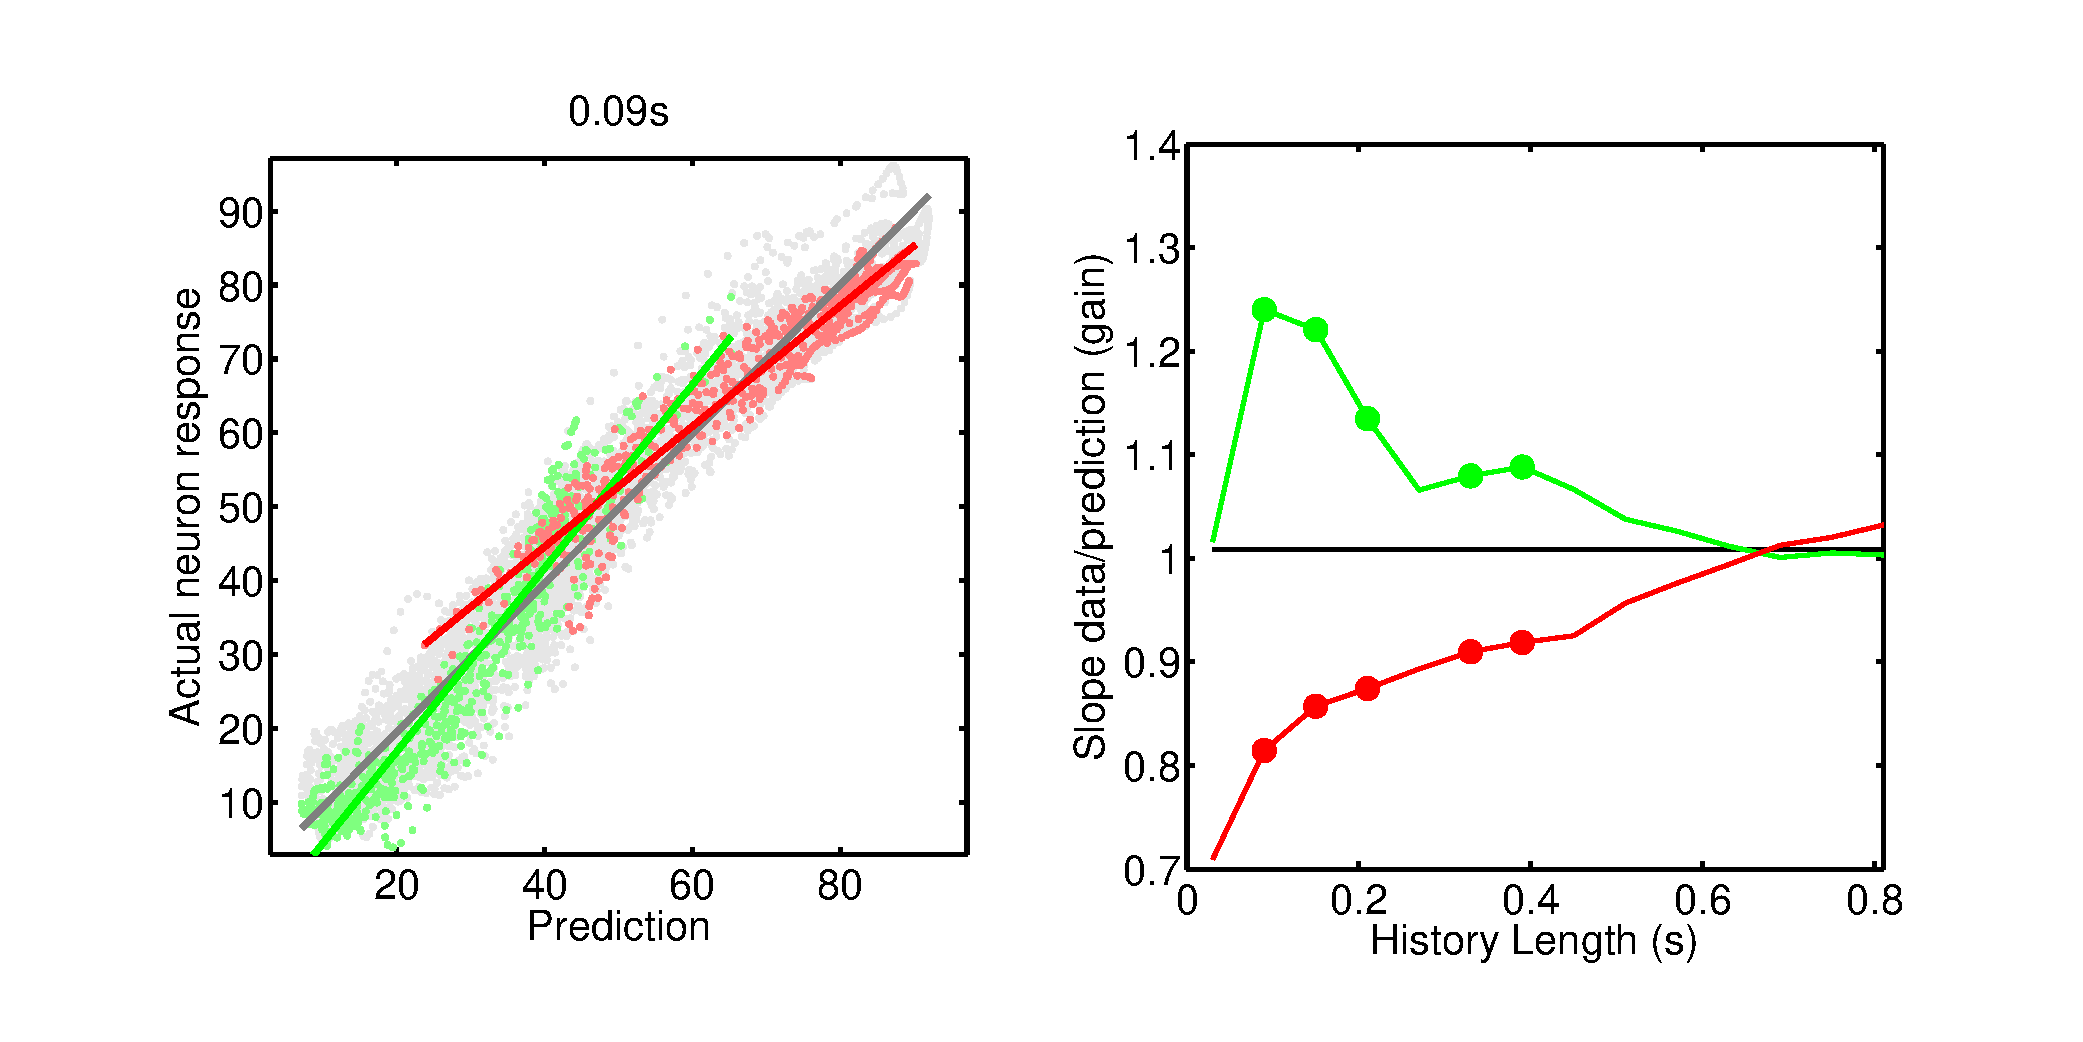
\includegraphics [width=\textwidth]{DA_Paper_04.pdf}
\begin{par}
We now repeat the analysis on a different data set, where the same odor is presented to the same type of neuron, but the flickering stimulus has a longer correlation time. The response of the neuron is now quite different, and sometimes goes to 0 (stops firing entirely).
\end{par} \vspace{1em}
\begin{par}
This data file is being used for this analysis:
\end{par} \vspace{1em}

        \color{lightgray} \begin{verbatim}final_2012_05_28_ab3A_1o3ol_randstim_100ms_60sec.mat
\end{verbatim} \color{black}
    \begin{par}
How is the filter changed? The following figure shows the filter computed from this dataset compared to previous dataset.
\end{par} \vspace{1em}

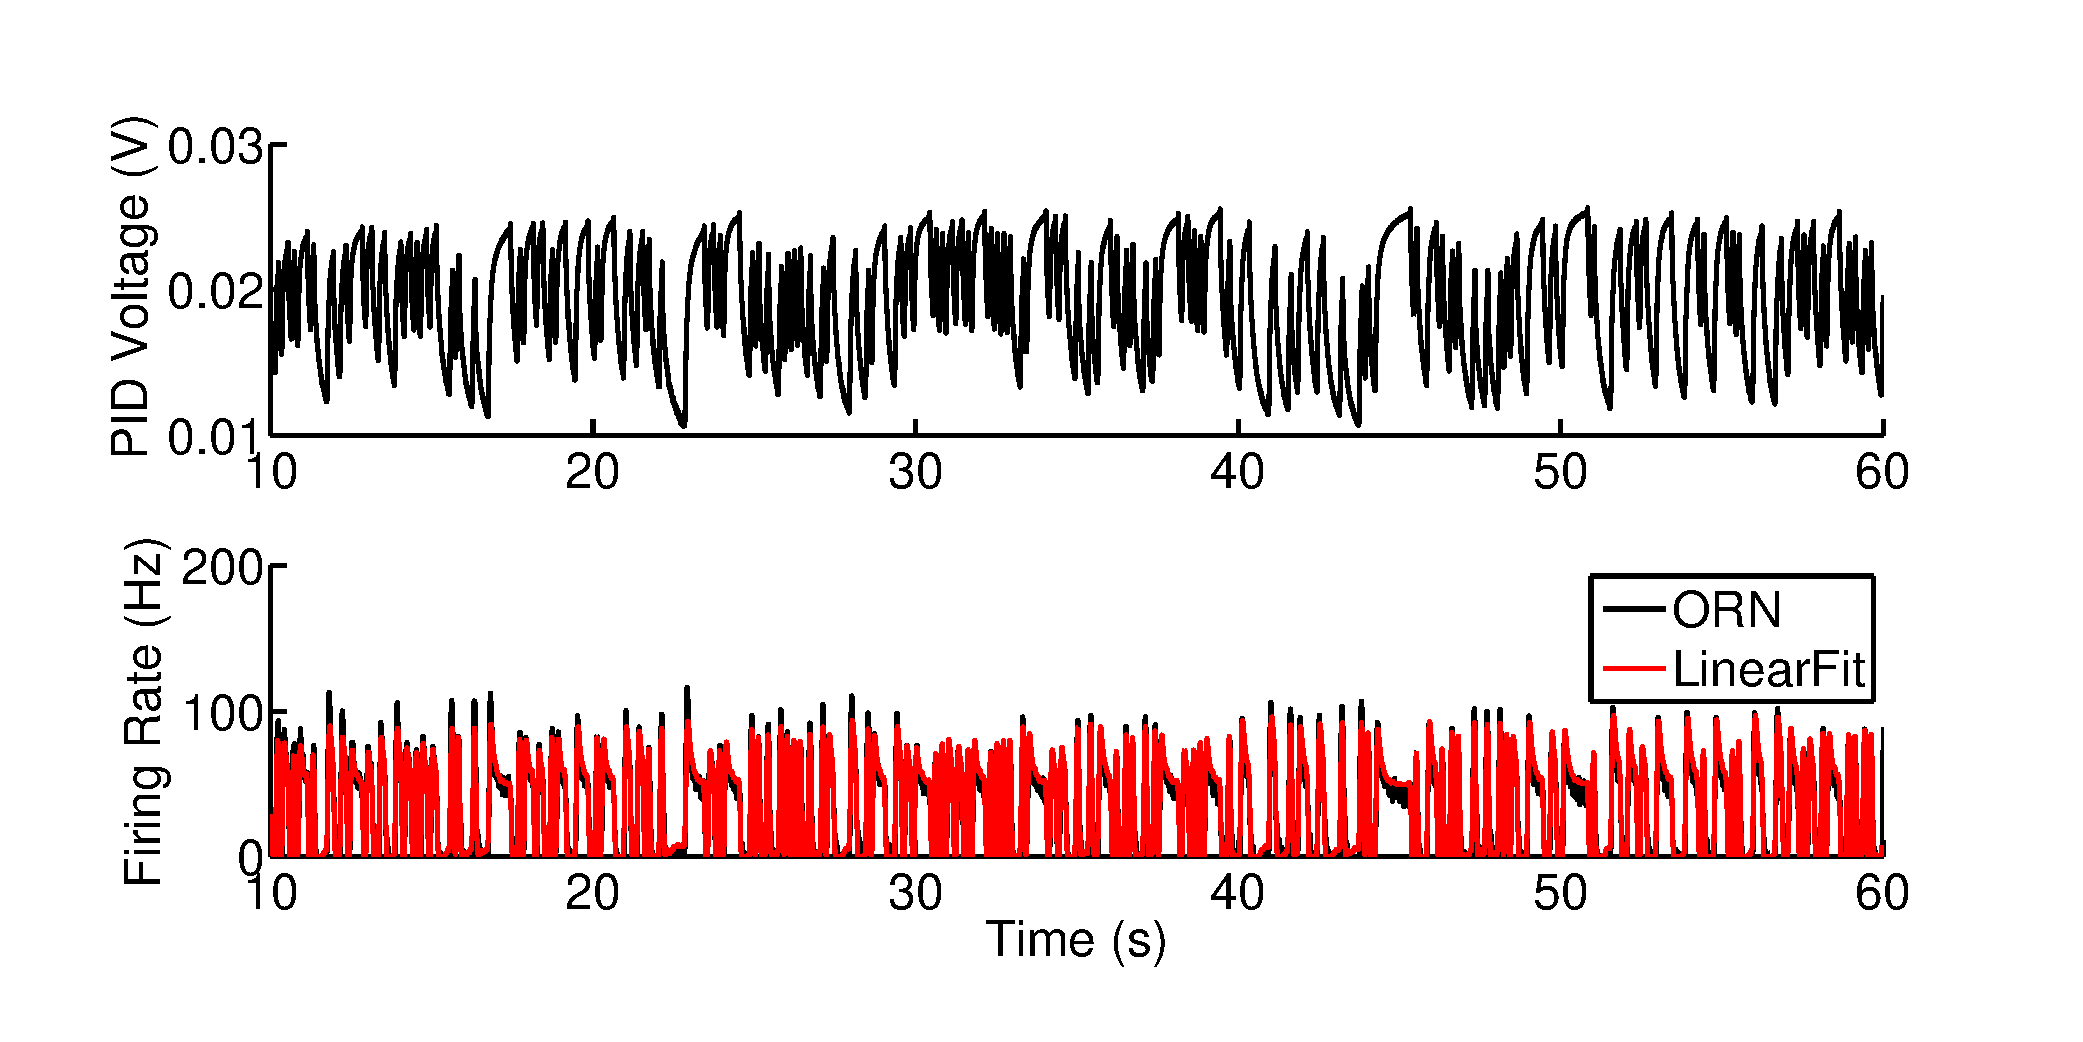
\includegraphics [width=\textwidth]{DA_Paper_05.pdf}

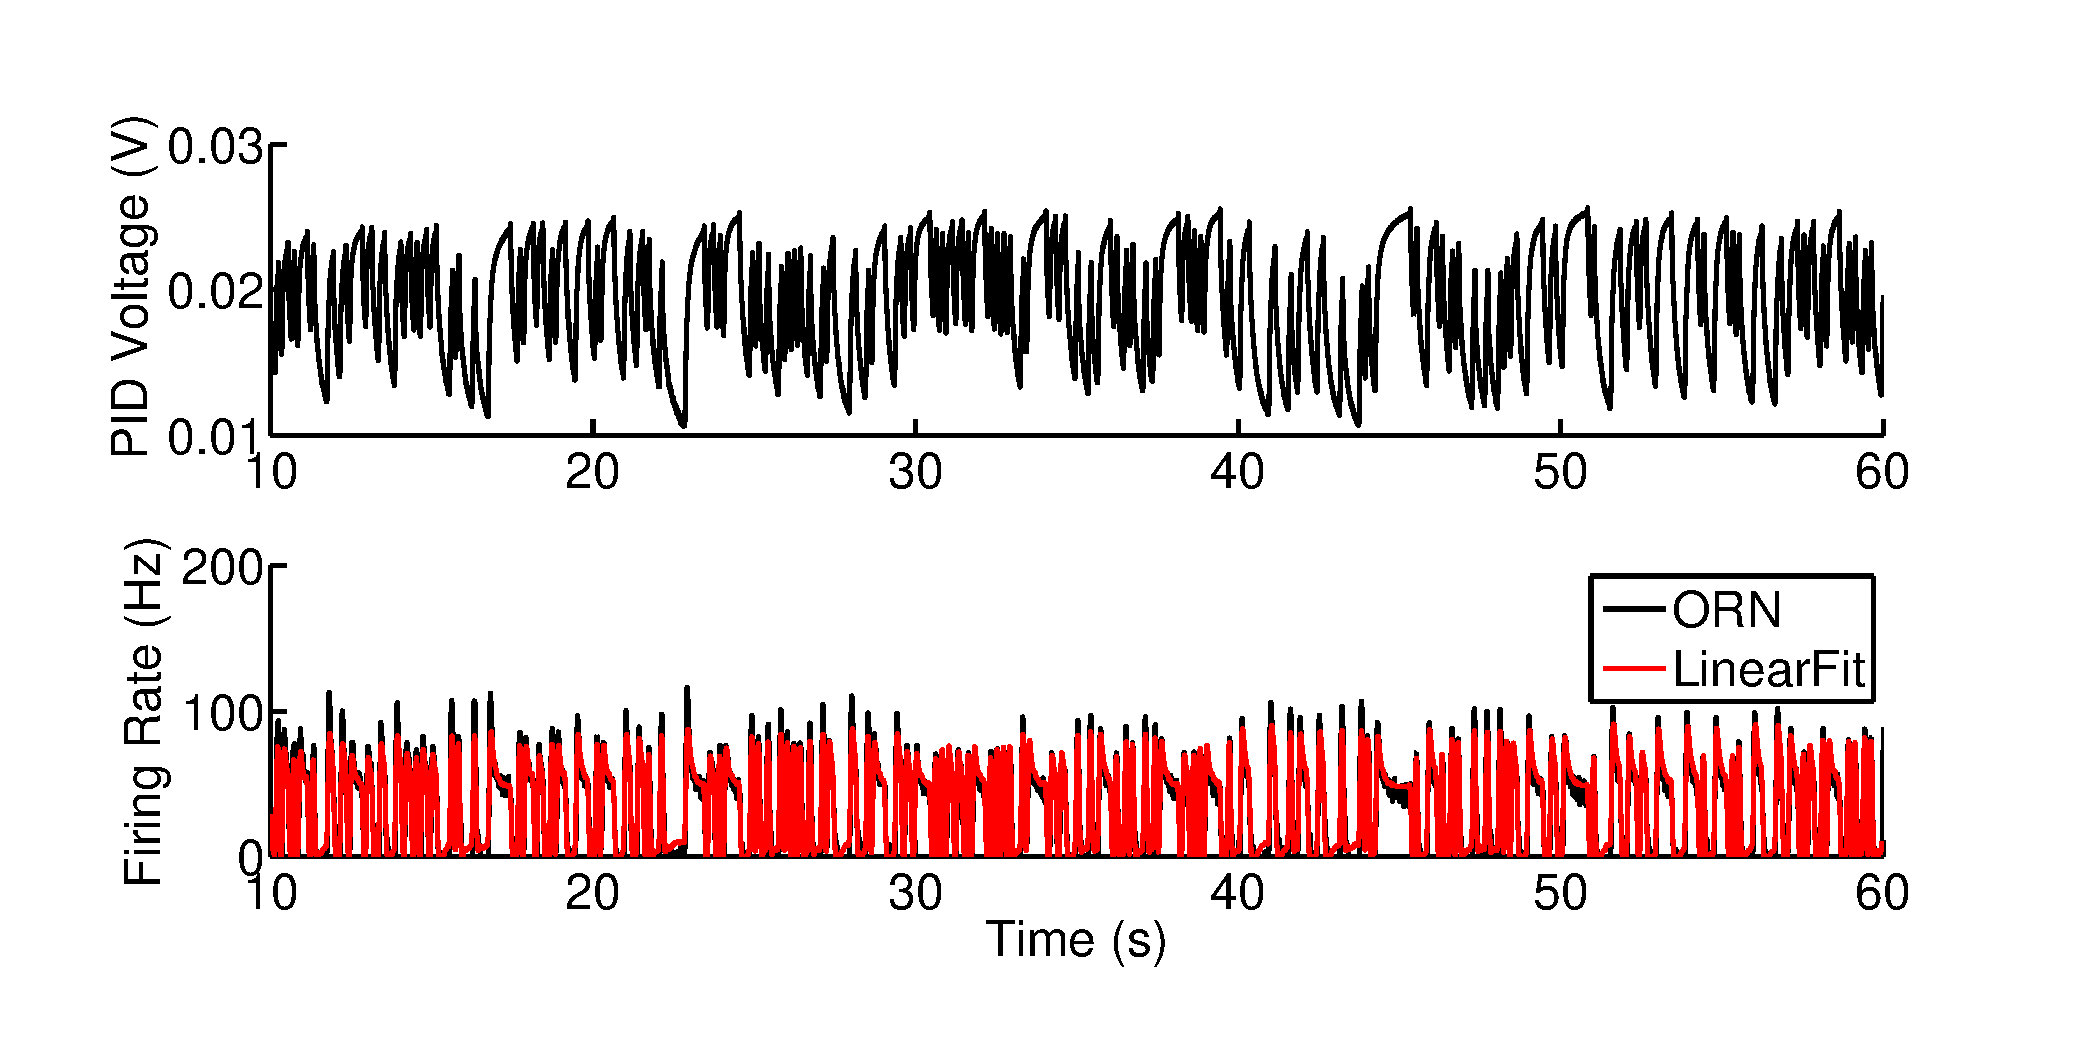
\includegraphics [width=\textwidth]{DA_Paper_06.pdf}

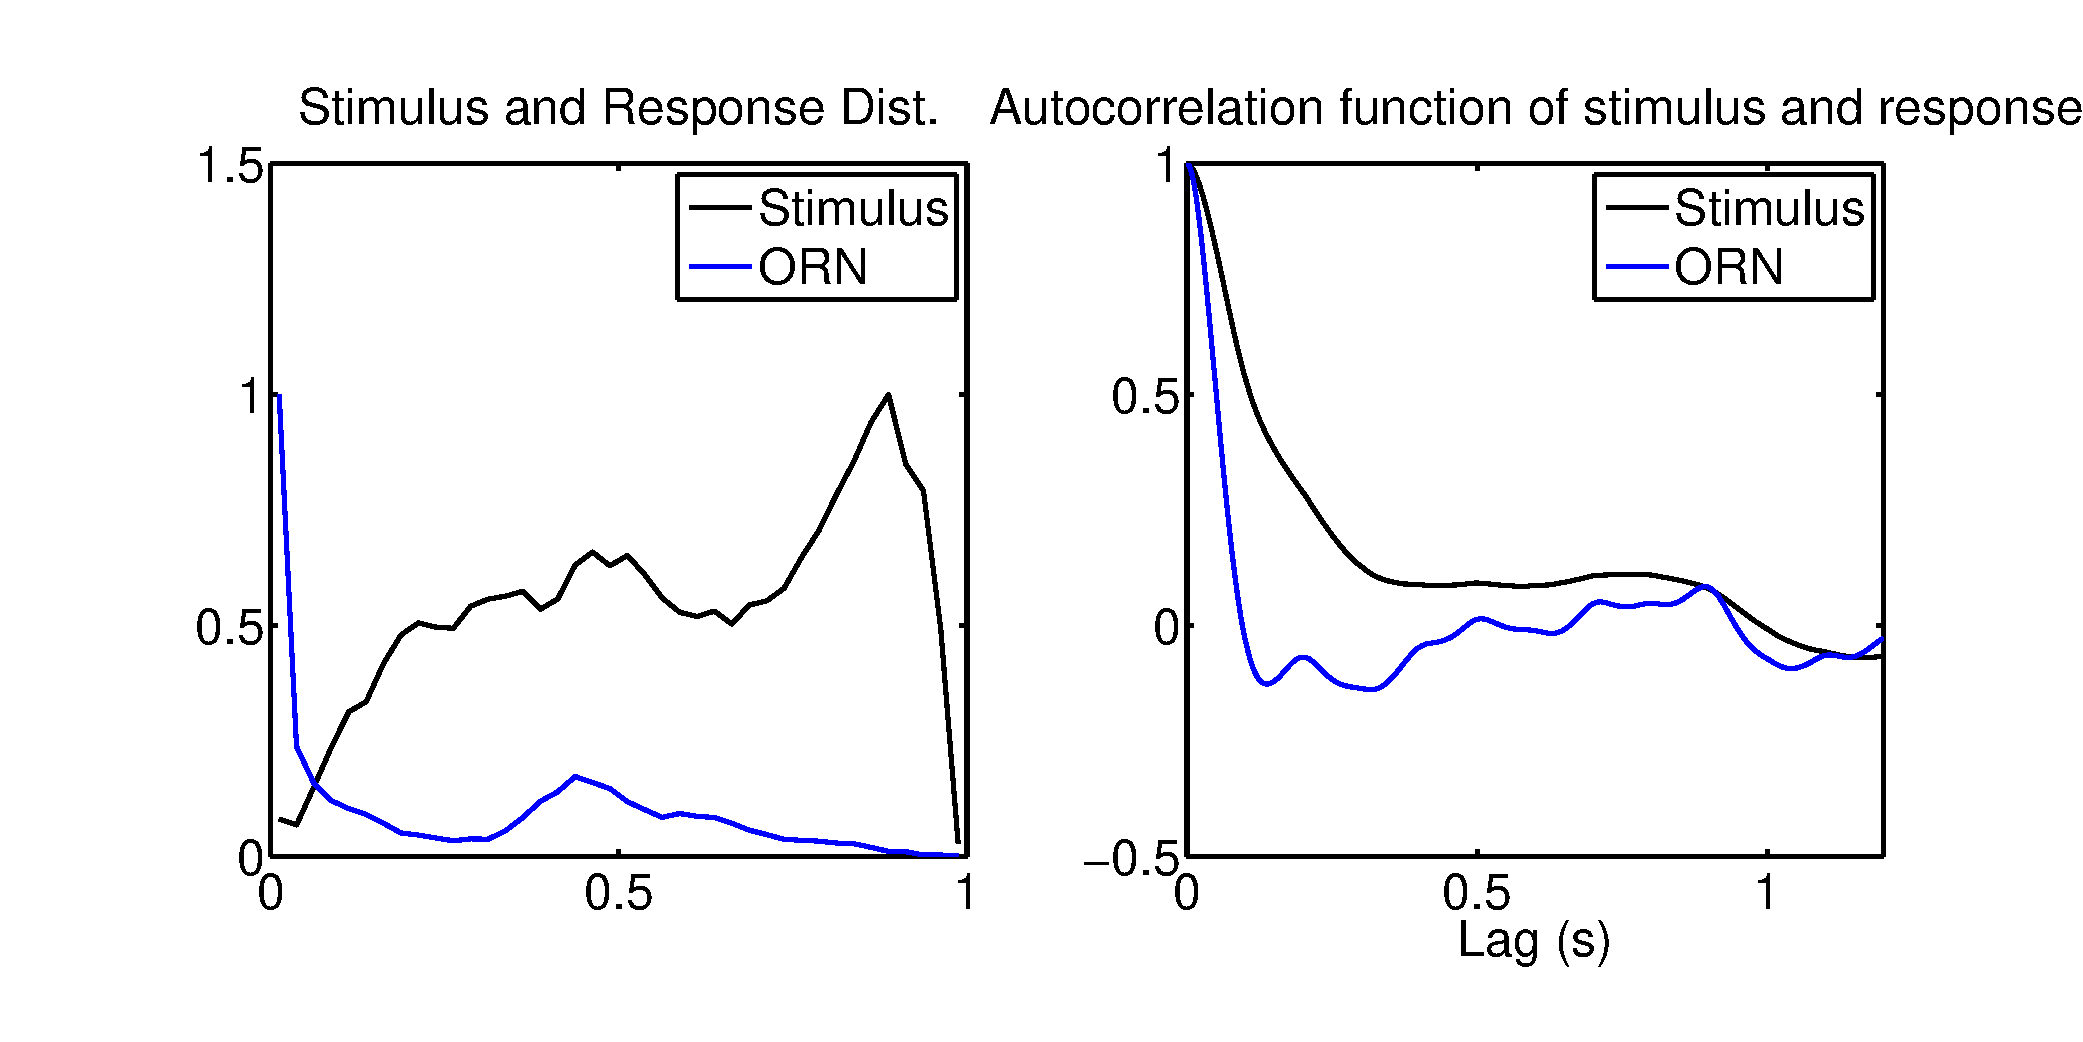
\includegraphics [width=\textwidth]{DA_Paper_07.pdf}

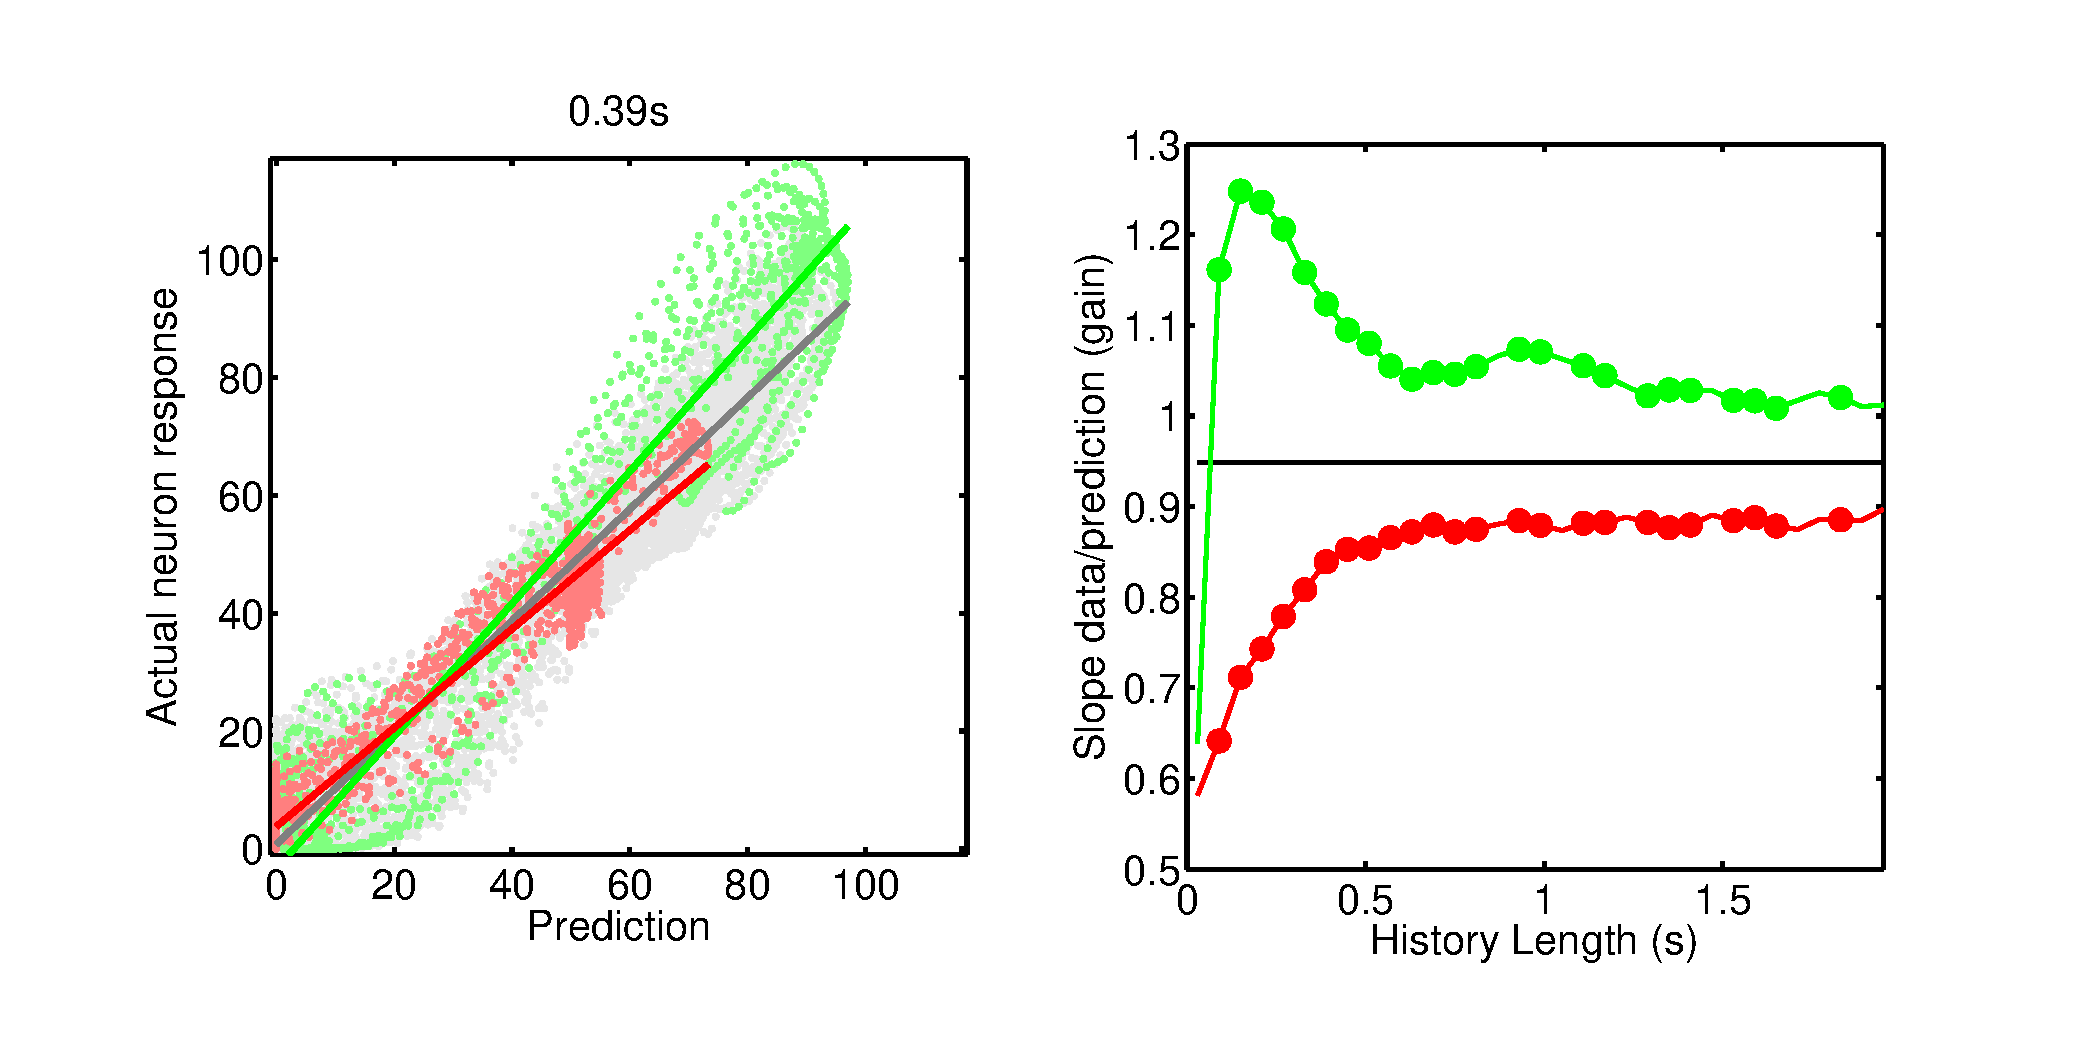
\includegraphics [width=\textwidth]{DA_Paper_08.pdf}


\subsection*{Can the DA Model account for fast adaptation?}

\begin{par}
Here we fit the DA model to the data.
\end{par} \vspace{1em}
\begin{par}
How does fast adaptation depend on odor type?
\end{par} \vspace{1em}
\begin{par}
Can the DA Model account for responses to pulses of odor?
\end{par} \vspace{1em}



\end{document}
    
